\section{Fundamentals}

\begin{frame}{Experiments}

    \begin{itemize}
        \item An \textbf{experiment}\footnote{In statistics an experiment is sometimes called a \emph{trial}} is a procedure carried out to validate or refute a \emph{hypothesis}.
        \item Typically, we study the relationships between some variables.
        \item Variables can be \emph{dependent} or \emph{independent}.
        \item \emph{Independent} variables\footnote{Other names: \emph{predictor/explanatory variables}, \emph{features}, \emph{covariates}} are manipulated by an experimenter. They're usually denoted as $X_i$ ($i \geq 1$).
        \item \emph{Dependent} variables\footnote{Other names: \emph{response/explained/outcome/output variables}, \emph{labels}} describe the event expected to change with the independent variables. They're usually denoted as $Y_i$ ($i \geq 1$). 
    \end{itemize}

\end{frame}

\begin{frame}{Experiments}

\begin{example}
    \medskip
    Try to design experiments aimed at:
    
    \begin{itemize}
        \item Proving that a coin is biased (e.g. it yields more tails than heads in tossing)?
        \item Finding how much airflow is required to maintain the CO$_2$ level in this room below 800 ppm.
        % Note that people breathe out different amounts of CO2
        \item Finding how much time devoted to statistics is required to get at least a 75\% chance of passing this course.
        % Draw a logistic regression curve
    \end{itemize}
    
\end{example}

\end{frame}

\begin{frame}{Data Types}
    \begin{figure}
        \includegraphics[width=0.75\textwidth]{gfx/variable_types}
    \end{figure}
    \begin{description}
        \item[Nominal] Variables with inherent order (categories)%, e.g. gender
        \item[Ordinal] Variables with ordered series%, e.g. performance
        \item[Binary] Variables with only two options%, e.g. coin tossing
        \item[Discrete] Variables with finite number of possible values%, e.g. number of damaged parts
        \item[Continuous] Variables with real numbers%, e.g. height, length
    \end{description}
\end{frame}

\begin{frame}{Data Types}

    \emph{Discuss in pairs:}
    \begin{enumerate}
        \item Think of some examples of nominal, ordinal, binary,
        discrete, and continuous data types in real life.
        \item Why do we distinguish discrete from nominal/ordinal/binary variables?
    \end{enumerate}


\end{frame}

\begin{frame}{Data Sample}

A \textbf{data sample} is a subset of a statistical population, selected according to some procedure. The elements of a sample are called \textbf{sample points} or \textbf{observations}.

Exemplary sampling methods:

\begin{itemize}
    \item Simple random sampling (SRS)
    \item Stratified sampling
    \item Cluster sampling
\end{itemize}

\end{frame}

\begin{frame}{Simple Random Sampling (SRS)}

\begin{columns}
    \begin{column}{0.5\textwidth}
        \begin{itemize}
            \item Each element has an equal probability of selection
            \item Variance between individual results within the sample is a good indicator of variance in the overall population
            \item Sample may not reflect the composition of the population (especially true for small samples)
        \end{itemize}
    \end{column}
    \begin{column}{0.5\textwidth}
        \includegraphics[width=\textwidth]{gfx/random_sampling}
    \end{column}
\end{columns}

\end{frame}

\begin{frame}{Stratified Sampling}

\begin{columns}
    \begin{column}{0.5\textwidth}
        \begin{itemize}
            \item Population is divided into independent categories, called \textit{strata}
            \item Random elements are selected from each \textit{stratum} and added to the sample
            \item Ensures that each \textit{stratum} is represented in the sample
            \item However, sometimes it is difficult to select relevant \textit{strata}
        \end{itemize}
    \end{column}
    \begin{column}{0.5\textwidth}
        \includegraphics[width=\textwidth]{gfx/stratified_sampling}
    \end{column}
\end{columns}

\end{frame}

\begin{frame}{Cluster Sampling}

\begin{columns}
    \begin{column}{0.5\textwidth}
        \begin{itemize}
            \item Population is divided into groups (\textit{clusters}), e.g. by geography
            \item Sample is composed of randomly selected \textit{clusters}
            \item Clustering can reduce travel and administrative costs (e.g. in the case of surveys)
            \item Larger samples required than in the case of SRS
        \end{itemize}
    \end{column}
    \begin{column}{0.5\textwidth}
        \includegraphics[width=\textwidth]{gfx/cluster_sampling}
    \end{column}
\end{columns}

\end{frame}

\begin{frame}{Probability}

    \begin{block}{Probability}
        \begin{itemize}
            \item Measure of the likehood that an event will occur
            \item Quantified between 0 (impossibility) and 1 (certainty)
            \item In a \emph{random} and \emph{well-defined} experiment it is calculated as the number of desired outcomes divided by the total number of all outcomes
        \end{itemize}
    \end{block}
    
    \begin{example}
        \smallskip
        When tossing a fair coin once, the probability P of getting an outcome of "head-head" is 0.25. There are 4 possible outcomes: "head-head", "head-tail", "tail-head", "tail-tail".
    \end{example}

\end{frame}

\begin{frame}{Probability}

    \begin{columns}
        \begin{column}{0.65\textwidth}
        Probability of getting a specific number N in rolling a six-sided die:
        \end{column}
        \begin{column}{0.25\textwidth}
        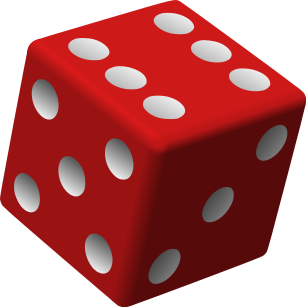
\includegraphics[width=0.45\textwidth]{gfx/web/die}
        \end{column}
    \end{columns}
    
    \begin{tabular}{l | r r r r r r}
        N & 1 & 2 & 3 & 4 & 5 & 6 \\
        \hline
        P(N) & $\frac{1}{6}$ & $\frac{1}{6}$ & $\frac{1}{6}$ & $\frac{1}{6}$ & $\frac{1}{6}$ & $\frac{1}{6}$ \\
    \end{tabular}
    
    \bigskip
    \begin{columns}
        \begin{column}{0.65\textwidth}
            Probability of getting a specific sum\\
            S = N$_1$ + N$_2$ in rolling two six-sided dice:
        \end{column}
        \begin{column}{0.25\textwidth}
            \includegraphics[width=\textwidth]{gfx/web/dice.png}
        \end{column}
    \end{columns}
    
    \begin{tabular}{l | r r r r r r r r r r r r}
        S & 1 & 2 & 3 & 4 & 5 & 6 & 7 & 8 & 9 & 10 & 11 & 12 \\
        \hline
        P(S) & 0 & $\frac{1}{36}$ & $\frac{2}{36}$ & $\frac{3}{36}$ & $\frac{4}{36}$ & $\frac{5}{36}$ & $\frac{6}{36}$ & $\frac{5}{36}$ & $\frac{4}{36}$ & $\frac{3}{36}$ & $\frac{2}{36}$ & $\frac{1}{36}$ \\
    \end{tabular}
    
    \medskip
    \begin{example}
        What are the possible outcomes (N$_1$, N$_2$) for S = 7?
    \end{example}

\end{frame}

\begin{frame}{Random Variable}
    \begin{block}{Random Variable}
    
    \begin{itemize}
    \item Outcome of a random process
    \item It has a probability distribution specifying the probability of each outcome
    \end{itemize}
    
    \begin{example}
    \medskip
    \emph{Tossing a coin} is a random process. The outcome (H or T) is a random variable. Each outcome has a specific probability of occurring (in this case 0.5, 0.5). The labels (H, T) can be replaced with numerical values, e.g. 0 and 1.
    \end{example}
    
    
    \end{block}
\end{frame}

\begin{frame}{Distribution}
    \begin{figure}
        \includegraphics[width=\textwidth]{R/plots/pdf}\\
        \includegraphics[width=\textwidth]{R/plots/pmf}
    \end{figure}
\end{frame}


\begin{frame}{Expected Value}
    Probability-weighted average for all possible values:
    \begin{equation}
        E(X) = x_1 p_1 + x_2 p_2 + ... + x_n p_n
    \end{equation}
    
    Arithmetic average in case of equally probable events:
    \begin{equation}
    E(X) = \frac{1}{N} \sum x_i
    \end{equation}
    
    \emph{Expected value} is sometimes called \emph{population mean} and denoted with $\mu$.
    
    \begin{example}
        \medskip
        What is the expected value in rolling a six-sided die?
    \end{example}
    %\pause
    %Answer: $(1+2+3+4+5+6) / 6 = 3.5$
\end{frame}

\begin{frame}{Expected Value for Continuous PDF}
    If $f(x)$ is the PDF of $X$, then
    
    \begin{equation*}
    E(X) = \int x \, f(x) dx
    \end{equation*}
    
    \begin{example}
        \medskip
        What is the expected value in the following cases?
        
        \includegraphics[width=\textwidth]{R/plots/expected_value_pdf_ex}
    \end{example}
\end{frame}

\begin{frame}{Test Data Set}

    Data set to be used when practicing calculations of standard deviation, variance, and covariance:
    
    \begin{center}
        \begin{tabular}{r r}
            X       &   Y \\
            \hline
            -1.24   &   -1.84 \\
            0.43    &   0.54 \\
            -0.65   &   -1.00 \\
            0.18    &   0.34 \\
            -0.57   &   -0.88
        \end{tabular}
    \end{center}

\end{frame}

\begin{frame}{Standard Deviation}
    \textbf{Standard deviation} is a measure of the dispersion of the data set, i.e. it quantifies how far the data points are from the mean.
    
    Sample standard deviation ($N < 30$):
    \begin{equation}
    s = \sqrt{\frac{\sum_{i=1}^{N} (x_i - \bar{x})^2}{N-1}}
    \end{equation}
    
    Population standard deviation (or sample if $N \geq 30$):
    \begin{equation}
    \sigma = \sqrt{\frac{\sum_{i=1}^{N} (x_i - \bar{x})^2}{N}}
    \end{equation}
    
    \begin{example}
        \medskip
        Calculate for X and Y from the test data set.
    \end{example}
\end{frame}

\begin{frame}{Standard Deviation}
    \begin{figure}
        \includegraphics[width=\textwidth]{R/plots/SD}
        Standard deviation in different data sets with the same mean
    \end{figure}
\end{frame}

\begin{frame}{Variance}
    \textbf{Variance} ($\text{Var}(X), \sigma^2, s^2$) is also a measure of the dispersion in the data set. It is the expected value of the squared deviation of a random variable from its mean:
    
    \begin{equation}
    \text{Var}(X) = \sigma^2 = E[(X - \mu)^2] = \frac{1}{N} \sum_{i=1}^{N}(x_i - \mu)^2
    \end{equation}
    
    \begin{example}
        \medskip
        Calculate for X and Y from the test data set.
    \end{example}
\end{frame}

\begin{frame}{Covariance}
    \textbf{Covariance} is a measure of the joint variability of two random variables.
    \begin{figure}
        \includegraphics[width=\textwidth]{R/plots/covariance}
    \end{figure}
\end{frame}

\begin{frame}{Covariance}
    \textbf{Covariance} is calculated as the expected product of deviations of $X$ and $Y$ from their individual expected values:   
    \begin{align}
    \text{Cov}(X, Y) &= E[(X - E[X])(Y - E[Y])] = \\
    &= \frac{1}{N} \sum_{i=1}^{N}(x_i - E[X])(y_i - E[Y])
    \end{align}
    
    \begin{example}
        \medskip
        Calculate Cov($X$, $Y$) based on the test data set.
    \end{example}
\end{frame}

\begin{frame}{Hands-on Training: R}

    \textbf{Part 1:} Guided by the teacher
    \begin{itemize}
        \item Calculating the mean, variance, standard deviation, covariance
        \item Data frames
    \end{itemize}

    \textbf{Part 2:} Own/home work
    \begin{itemize}
        \item Read {\small \url{https://www.tutorialspoint.com/r/r_data_types.htm}}
        \item Read {\small \url{https://www.tutorialspoint.com/r/r_variables.htm}}
        \item Read {\small \url{https://www.tutorialspoint.com/r/r_operators.htm}}
    \end{itemize}

\end{frame}